\documentclass{sig-alternate}

\usepackage{fourier}
\usepackage[scaled]{beramono}
\usepackage[T1]{fontenc}
\usepackage{pgfplots}
\usepackage{listings}

\begin{document}

\title{Metropolis-Hastings Algorithm and Gibbs Sampling Scaling on
Bayesian networks for Marginalization Queries}
\author{
	Gio Borje \#41894135\\
	\affaddr{University of California, Irvine} \\
	\email{gborje@uci.edu}}
\maketitle

\begin{abstract}
We analyze the Metropolis-Hastings algorithm relative to Gibbs sampling
algorithm on Bayesian networks for solving for inference queries involving
marginalization.
\end{abstract}

\section{Introduction} % (fold)
\label{sec:Introduction}
	Markov Chain Monte Carlo (MCMC) methods are frequently used to sample
	from a complex target distribution in order to resolve approximation
	queries such as for expected values and marginalized probabilities.
	The MCMC methods are applied to Bayesian networks. The Bayesian
	network is represented as a graph where each node represents a random
	variable and the edges of the graph represent conditional
	relationships between variables. \cite{rn2010}

	Since exact inference is intractable, we only compare approximation
	methods for our analysis. In this analysis, we compare the running
	time of the Metropolis-Hastings algorithm to the Gibbs sampling
	algorithm. Because Gibbs sampling is a special case of
	Metropolis-Hastings' algorithm, we expect Gibbs sampling to run
	quicker. This paper will proceed as follows. Section 2 will describe
	our sampling methods as well as benchmarking methods. Section 3 will
	demonstrate our results of the three algorithms. Finally, we discuss
	these results in section 4.
% section Introduction (end)

\section{Methods} % (fold)
\label{sec:Methods}
	\begin{figure}[!htbp]
		\centering
		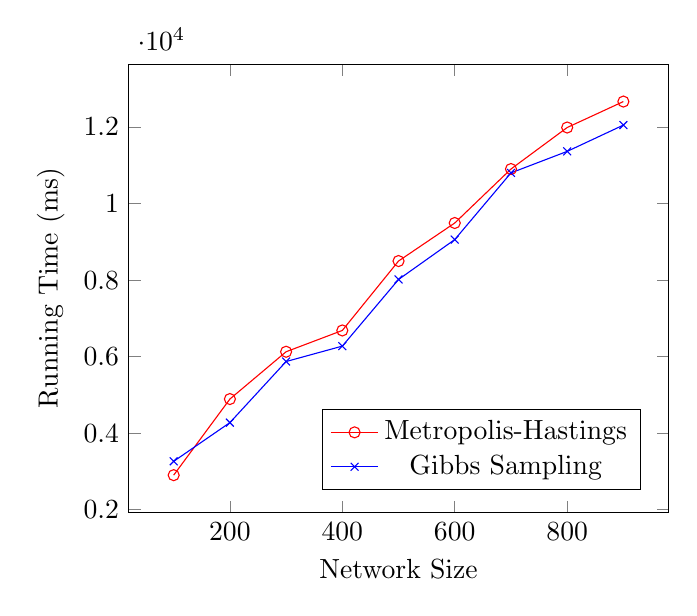
\begin{tikzpicture}
			\begin{axis}[domain=100:900, xlabel={Network Size}, ylabel={Running Time (ms)},
			legend style={
			at={(0.95,0.05)},
			anchor=south east}]
			\addplot[mark=o, color=red]
				coordinates {
					(100,2903)
					(200,4892)
					(300,6128)
					(400,6684)
					(500,8498)
					(600,9492)
					(700,10902)
					(800,11987)
					(900,12665)
				};
			\addlegendentry{Metropolis-Hastings}

			\addplot[mark=x,color=blue]
				coordinates {
					(100,3264)
					(200,4276)
					(300,5872)
					(400,6275)
					(500,8016)
					(600,9059)
					(700,10801)
					(800,11363)
					(900,12050)
				};
			\addlegendentry{Gibbs Sampling}
			\end{axis}
		\end{tikzpicture}
	\label{fig:results}
	\caption{Metropolis-Hastings vs. Gibbs Sampling Running Time on Bayesian Networks}
	\end{figure}

	\begin{table*}[ht]
		\centering
		\begin{tabular}{|l|l|l|l|l|l|l|l|l|l|}
		\hline
		\textbf{Network Size}
			& 100 & 200 & 300 & 400 & 500 & 600 & 700 & 800 & 900 \\\hline
		\textbf{Metropolis-Hastings (ms)} 
			& 2903 & 4892 & 6128 & 6684 & 8498 & 9492 & 10902 & 11987 &12665 \\\hline 
		\textbf{Gibbs Sampling (ms)} 
			& 3264 & 4276 & 5872 & 6275 & 8016 & 9059 & 10801 & 11363 & 12050 \\\hline
		\end{tabular}
		\label{tab:running_time}
		\caption{Running time in milliseconds of three marginalization queries
		on Bayesian networks of increasing size}
	\end{table*}

	\subsection{System Architecture} % (fold)
	\label{sub:System Architecture}
		We operate on a Bayesian network implementation in C++11 using only standard
		libraries. We test the correctness of the Bayesian network for simple operations
		such as adding new nodes and querying for marginal probabilities on individual
		random variables through a custom unit testing library. We have also
		implemented a simple benchmarking library based on the STL's steady
		clocks for measuring the running time of a query in milliseconds.

		Creating a Bayesian network requires two type parameters which
		default to integer values. The type parameters are the
		\lstinline$NodeType$ and \lstinline$ValueType$ which can be
		interpreted as the type of the node label and the type of values
		that the node can take on. Adding nodes to the Bayesian network
		requires at least two parameters: \lstinline$node_id$ of type
		\lstinline$NodeType$ and a \lstinline$cpt$ of type
		\lstinline$CondProb$.

		The Bayesian network is primarily static and may only add nodes
		when its parent nodes have been added already. This is because
		conditional probability tables requires information regarding all
		possible parent node value combinations.
		
		Each conditional probability table is wrapped by the
		\lstinline$CondProb$ class which is capable of finding the
		appropriate distribution given a vector of parent values. Note
		that construction of a conditional probability table simply
		requires a map from a vector of a node's parents potential values
		to a probability distribution over the values of a node.
	% subsection System Architecture (end)


	\subsection{Benchmarking Architecture} % (fold)
	\label{sub:Benchmarking Architecture}
		Each benchmark is tested on three queries on a simple Bayesian network
		architecture. That is, for a network of size $N$, we have $N$ independent
		nodes of boolean value and single node that can take of $N$ values.
		Simply, this is the architecture of a multiplexer which is easy to test.

		We benchmark for increasing network sizes starting from size $100$ to size
		$900$ with four marginalization queries for checking if the final node has
		a specified value which is one of the elements in the set $\{8, 16, 32,
		64\}$. For both algorithms, the burn in time is specified to be at $32$
		and the number of samples taken is $512$.

		Due to the deterministic nature of the benchmarks, we simply use
		the metropolis update. For future work, we will enable
		parameterization on both the proposal distribution and the
		acceptance criteria for the algorithm.
	% subsection Benchmarking Architecture (end)

% section Methods (end)

\section{Results} % (fold)
\label{sec:Results}

The benchmark data set can be found in table \ref{tab:running_time} and
the data can be visualized in figure \ref{fig:results}. It is evident that
the Gibbs sampling algorithm is marginally faster than the
Metropolis-Hastings algorithm.

The running time of both algorithms grows approximately linearly relative
to the size of the network

% section Results (end)

\section{Discussion} % (fold)
\label{sec:Discussion}
	We speculate that the marginal difference in the computational time
	between Metropolis-Hastings and Gibbs sampling exists because the
	Metropolis-Hastings algorithm requires computation of an acceptance ratio
	for its update mechanism whereas Gibbs sampling does not require
	computation of an acceptance ratio.
	
	Since the standard deviation of the Metropolis-Hastings running time
	is approximately $463$ ms from the Gibbs sampling running time,
	we estimate that half a second is the cost of computing the acceptance
	ratio where the bottleneck is computing the probability of a specified
	Bayesian network configuration of an order of magnitude of three in
	size.
% section Discussion (end)

\bibliographystyle{plain}
\bibliography{sources}

\end{document}
